\begin{frame}[fragile]
\frametitle{Concrete Syntax for Our Extension Layer}
\begin{itemize}
\item For bidirectional pragmatic-to-strict translation
\item $\extension{e}{\lflam[E_1]{x_1}\ldots\lflam[E_n]{x_n}\sigfr{\Sigma}}$ is written as 

%\begin{block}{}
%\vspace{-.5em}
\begin{center}
\begin{lstlisting}
<extension name="$e$">
 <parameter name="$x_1$">$E_1$</parameter>
  $\hspace{2cm}\vdots$
  <parameter name="$x_n$">$E_n$</parameter>
  <theory>
      $\Sigma$
  </theory>
</extension>
\end{lstlisting}
\end{center}
%\end{block}
\vspace{.5em}
\item $\pragmatic{c}{e\;A_1\ldots A_n}$ is written as 
%\begin{block}{}
%\vspace{-.5em}
\begin{center}
\begin{lstlisting}
<pragmatic name="$c$" extension="$\mmturi{e}$">
    $A_1\ldots A_n$
</pragmatic>
\end{lstlisting}
\end{center}
%\end{block}

{\footnotesize $\mmturi{e}$ denotes $e$'s URI.}
\end{itemize}
\end{frame}

%\llquote{M}
%$\om{E_1}\ldots\om{E_n}$
%$\hspace{.45cm}\om{\Sigma}$
%<parameter name="$x_1$">$\om{E_1}$</parameter>


\begin{frame}
\frametitle{Pragmatic Surface Syntax}
\begin{itemize}
%\item A human-oriented syntax closer to notational convensions
\item Notation parser specific to each pragmatic surface syntax 
\lec{ongoing work for our Twelf surface syntax}
\lec{done for our sTeX surface syntax}
\end{itemize}

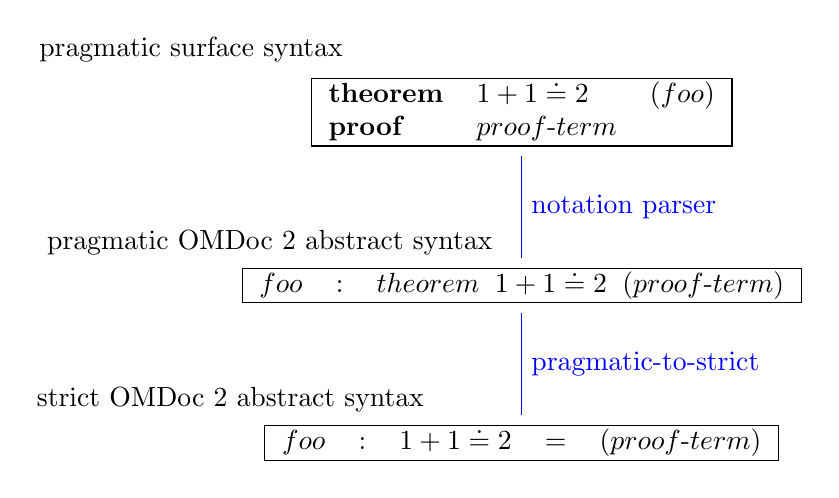
\begin{tikzpicture}
\node(n) at (4,4.2) {
\begin{tabular}{|lll|}\hline
\textbf{theorem} & $1 + 1 \doteq 2$ & $(foo)$ \\
\textbf{proof}   & $proof\textrm{-}term$ &\\
\hline
\end{tabular}
};

\node at (-.2,5) {\alert{pragmatic surface syntax}};
\node at (.8,2.55) {\alert{pragmatic OMDoc 2 abstract syntax}};
\node at (.3,.55) {\alert{strict OMDoc 2 abstract syntax}};
\node(p) at (4,2) {
\begin{tabular}{|lll|}\hline
$foo$ &:& $theorem\;\;1 + 1 \doteq 2\;\;(proof\textrm{-}term)$\\\hline
\end{tabular}
};

\node(s) at (4,0) {
\begin{tabular}{|lllll|}\hline
$foo$ &:& $1 + 1 \doteq 2$ &=& $(proof\textrm{-}term)$\\\hline
\end{tabular}
};

\draw[blue,-\arrowtip] (n) --node[right] {notation parser} (p);
\draw[blue,-\arrowtip] (p) --node[right] {pragmatic-to-strict} (s);
\end{tikzpicture}
%\begin{tabular}{|lll|}\hline
%\textbf{theorem} & $1 + 1 \doteq 2$ & (foo) \\
%\textbf{proof}   & proof-term &\\
%\hline
%\end{tabular}
\end{frame}